\section{Load, Store and Branch Instructions}

\begin{figure}[h!]
	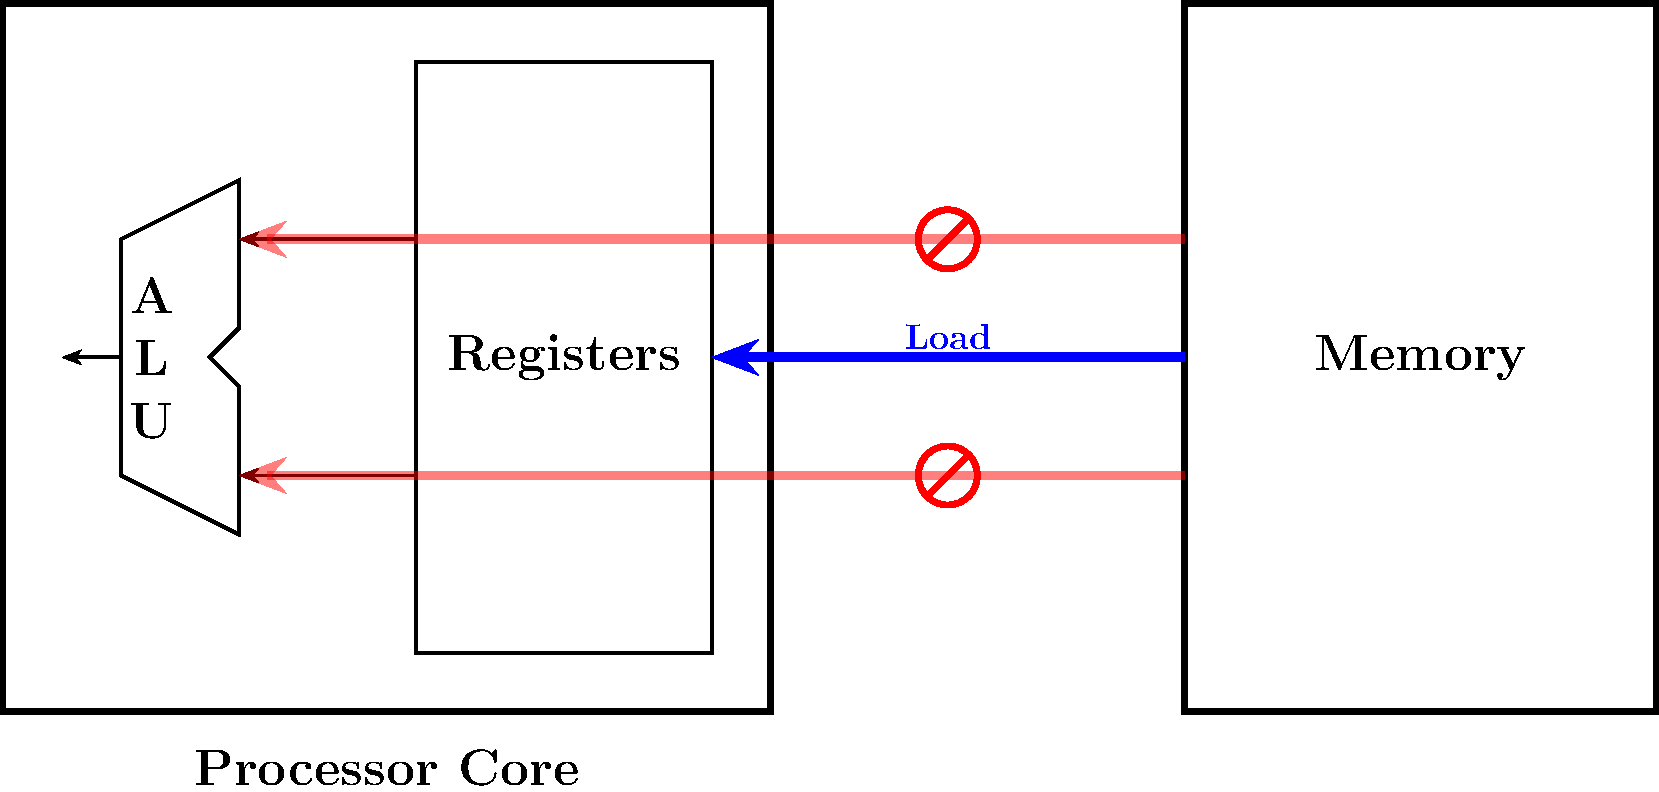
\includegraphics[width=\textwidth]{architectures/load.pdf}
	\caption{Loading Data from Memory}
\end{figure}

\begin{figure}[h!]
	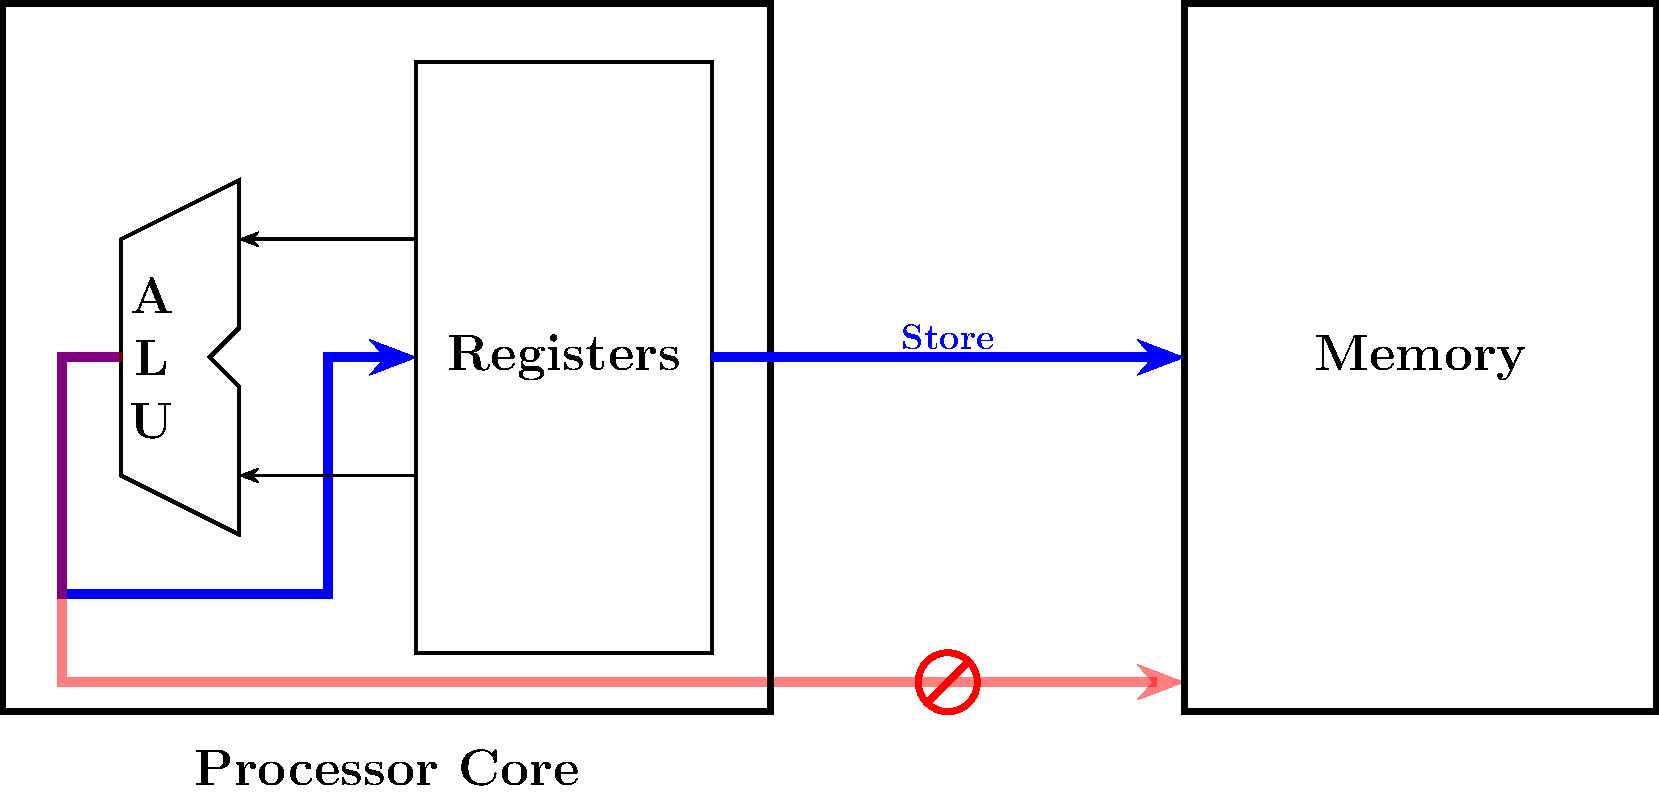
\includegraphics[width=\textwidth]{architectures/store.pdf}
	\caption{Storing Data to Memory}
\end{figure}

\subsection{CPU components and Data paths}
\subsection{AArch64 User Registers}
\begin{itemize}
	\item General purpose registers
	\item Frame pointer
	\item PSTATE register
	\begin{itemize}
		\item Negative
		\item Zero
		\item Carry
		\item oVerflow
	\end{itemize}
	\item Link register
	\item Stack pointer
	\item Zero register
	\item Program counter
\end{itemize}

\subsection{Instruction Components}

\newpage
\subsubsection{Setting and using condition flags}

\begin{example}
\ \begin{table}[h!]\setstretch{1.25}\centering\ttfamily
\caption{Operation Examples}
\begin{tabular*}{\textwidth}{@{\extracolsep{\fill}} c|c||c|c|c|c}
	\toprule[1.2pt]
	\textbf{Operation} & \textbf{Result} & N & Z & C & V \\ \hline
	0x70000000 + 0x70000000 & 0xE0000000 & 1 & 0 & 0 & 1 \\ \hline
	0x80000000 + 0x80000000 & 0x00000000 & 0 & 1 & 1 & 1 \\ \hline
	0x90000000 + 0x90000000 & 0x30000000 & 0 & 0 & 1 & 1 \\ \hline
	0x00001234 - 0x00001000 & 0x00000234 & 0 & 0 & 1 & 0 \\ \hline
	0xFFFFFFFF - 0xFFFFFFFC & 0x00000003 & 0 & 0 & 1 & 0 \\ \hline
	0x80000005 - 0x80000004 & 0x00000001 & 0 & 0 & 1 & 0 \\ \hline
	0x70000000 - 0xF0000000 & 0x80000000 & 1 & 0 & 0 & 1 \\ \hline
	0xA0000000 - 0xA0000000 & 0x00000000 & 0 & 1 & 1 & 0 \\
	\bottomrule[1.2pt]	
\end{tabular*}
\end{table}
\end{example}

Let \begin{align*}
a = a_{31}a_{30}\cdots a_1a_0\in\mathbb{F}_2^{32}\\
b = b_{31}b_{30}\cdots b_1b_0\in\mathbb{F}_2^{32}\\
c = b_{31}c_{30}\cdots c_1c_0\in\mathbb{F}_2^{32},
\end{align*} where $c= a + b\bmod 2^{32}$.
\begin{table}[h!]\setstretch{1.25}\centering
\caption{Flag bits \texttt{NZCV} in \texttt{PSTATE}.}
\begin{tabular*}{\textwidth}{@{\extracolsep{\fill}} c|c|c|c}
	\toprule[1.2pt]
	\multicolumn{2}{c|}{\textbf{Name}} & \textbf{Logical Instruction} & \textbf{Arithmetic Instruction} \\ \cline{0-3}
	\texttt{N} & (Negative) & No meaning & $\texttt{N}=c_{31}$ \\ \cline{0-3}
	\texttt{Z} & (Zero) & Result is all zeroes & $\texttt{Z}=\bigoplus_{i=0}^{31}c_i=0$ \\ \cline{0-3}
	\texttt{C} & (Carry) & - & $\texttt{Z}=\bigoplus_{i=0}^{31}c_i=0$ \\ \cline{0-3}
	\texttt{V} & (oVerflow) & - & $\texttt{Z}=\bigoplus_{i=0}^{31}c_i=0$
\end{tabular*}
\end{table}

\begin{table}[h!]\setstretch{1.25}\centering
\caption{AArch64 condition modifiers.}
\resizebox*{\textwidth}{!}{\begin{tabular}{c|l|c|c}
	\toprule[1.2pt]
	\textbf{Condition Code} & \textbf{Meaning} & \textbf{Condition Flags} & \textbf{Binary Encoding} \\ \hline
	\texttt{EQ} & Equal & $\texttt{Z}=1$ & \texttt{0000} \\
	\texttt{NE} & Not Equal & $\texttt{Z}=0$ & \texttt{0001} \\ \hline
	\texttt{HI} & Unsigned Higher & $(\texttt{C}=1)\land(\texttt{Z}=0)$ & \texttt{1000} \\
\end{tabular}}
\end{table}
\subsubsection{Immediate Values}

\begin{terminology*}
An \textbf{immediate value} in assembly language is a \textit{constant value} that is specified by the programmer.
\end{terminology*}

There are two ways that immediate values can be specified in GNU ARM assembly:
\begin{description}
	\item[(Method 1)] The first way is as a literal immediate value. This can be optionally prefixed with a pound sign for clarity: \begin{center}
		\ttfamily \#<immediate|symbol>
	\end{center}
	\item[(Method 2)] The second way is the \begin{center}
		\ttfamily =<immediate|symbol>
	\end{center} syntax, which can only be used with the `\texttt{ldr}' pseudo-instruction.
\end{description}
\begin{table}[h!]\setstretch{1.25}\centering
\caption{Summary of Valid Immediate Values}
\resizebox*{\textwidth}{!}{\begin{tabular}{c|c|c|c|c}
	\toprule[1.2pt]
	\textbf{Immediate Type} & \textbf{Bits} & \textbf{Description} & \textbf{Legal} & \textbf{Illegal} \\
	Arithmetic & 12 & \\
	Logical & 13 & \\
\end{tabular}}
\end{table}

\newpage
\subsubsection{Addressing Modes}

\begin{table}[h!]\setstretch{1.25}\centering
\caption{Load/Store Memory Addressing Modes}
\resizebox*{1\textwidth}{!}{\begin{tabular}{l|l|l}
	\toprule[1.2pt]
	\textbf{Name} & \textbf{Syntax} & \textbf{Range} \\ \hline
	Register Address & \texttt{[Xn|sp]} & \\
	Singed Immediate Offset & \texttt{[Xn|sp, \#$\pm$<imm9>]} & $\intco{-2^8,2^8}$ \\
	Unsinged Immediate Offset & \texttt{[Xn|sp, \#<imm12>]} & $\intcc{\texttt{0},\texttt{0x7ff8}}$ \\
	Pre-indexed Immediate Offset & \texttt{[Xn|sp, \#$\pm$<imm9>]!} & $\intco{-2^8,2^8}$ \\
	Post-indexed Immediate Offset & \texttt{[Xn|sp], \#$\pm$<imm9>} & $\intco{-2^8,2^8}$ \\
	Register Offset & \texttt{[Xn|sp, Xm, (U|S)XTW]} & (or \texttt{LSL} \#1-3) \\
	Literal & \texttt{label} & $\pm 1$ MB\\
	Pseudo Load & \texttt{=<immediate|symbol>} & 64 bits \\
	\bottomrule[1.2pt]
\end{tabular}}
\end{table}
\vfill\nonumsidenote{\ \\ \ \\
\ttfamily ldr\hspace{1cm} \color{blue}x3\color{black}, \color{red}[x2]\color{gray} \\ \ \\
\color{gray} x3 = memory.word[x2] \\ \ \\
`ldr' stands for Load to Register \\
\ \\ \ \\
\color{black} str\hspace{1cm} \color{blue}x3\color{black}, \color{red}[x2]\color{gray} \\ \ \\
\color{gray} memory.word[x2] = x3 \\ \ \\
`str' stands for Store Register
}
\begin{figure}[h!]
	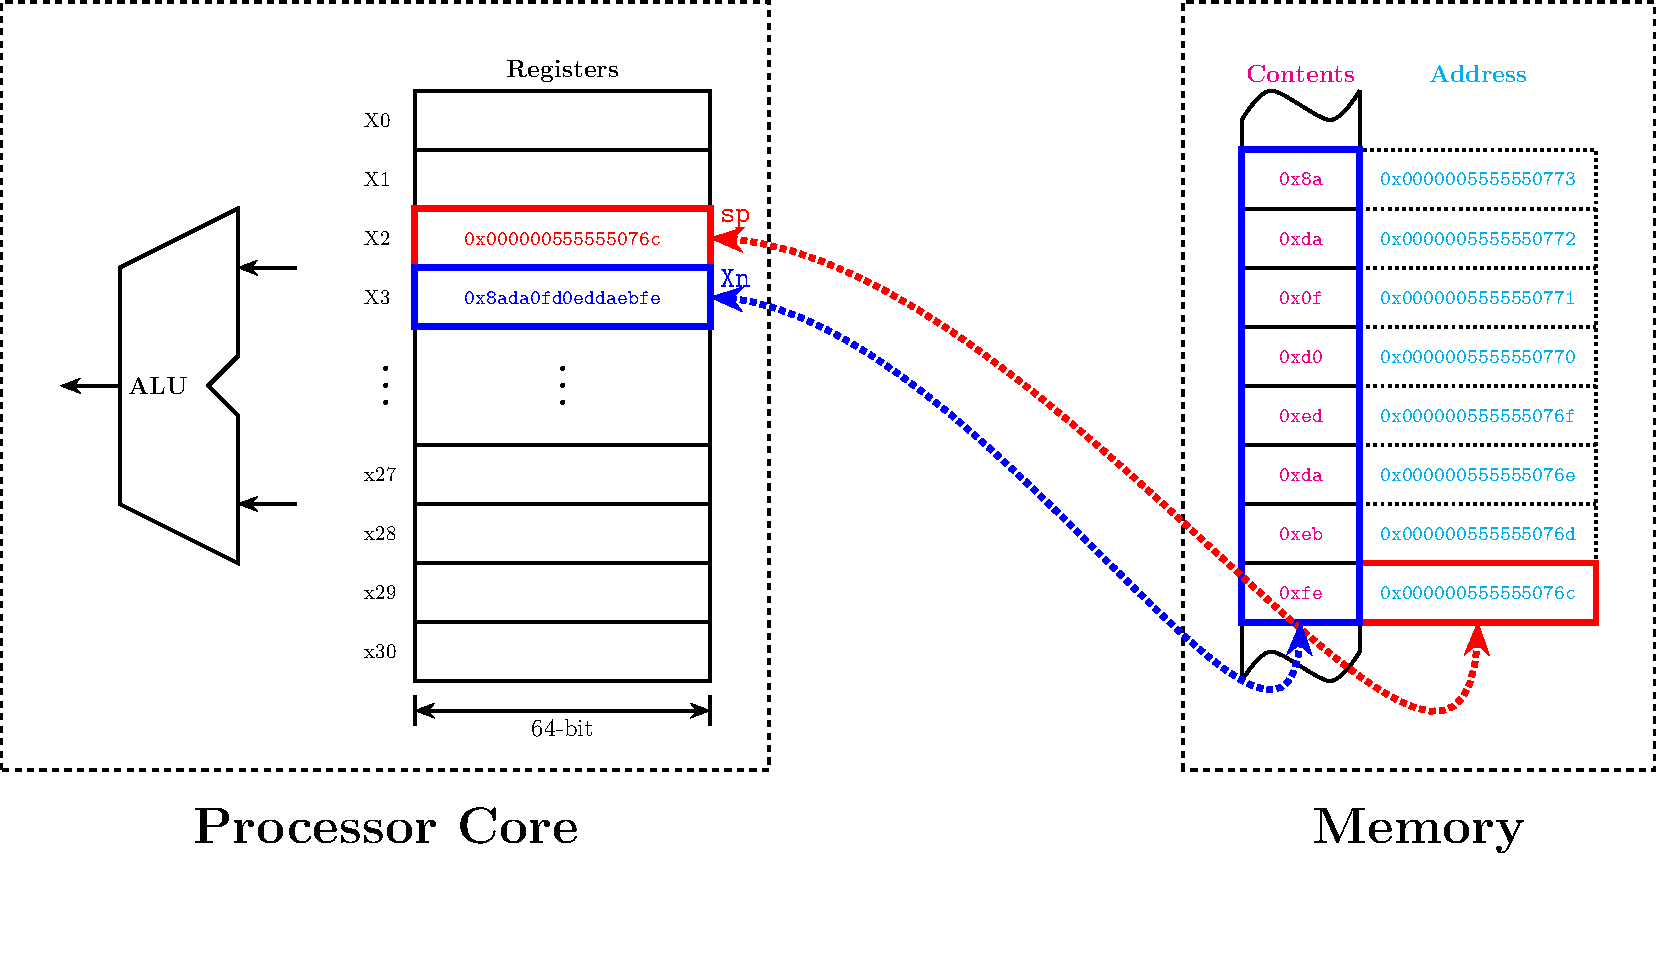
\includegraphics[width=\textwidth]{architectures/register-address.pdf}
	\caption{Access the memory address containing in the
		register \texttt{Xn} or \texttt{sp}.}
\end{figure}
\vfill
\begin{remark*}
	\texttt{[Xn]} or \texttt{[sp]} is just shorthand notation for $\texttt{[Xn,\ \#00]}\ \text{or}\ \texttt{[sp,\ \#00]}$, respectively.
\end{remark*}

\newpage
\nonumsidenote{\ \\ \ \\
	\ttfamily ldur\hspace{.5cm} \color{blue}x0\color{black}, \color{red}[x1, \#0x08] \\ \ \\
	\color{black} stur\hspace{.5cm} \color{blue}x0\color{black}, \color{red}[x1, \#-0x08]\color{gray} 
}
\begin{figure}[h!]
	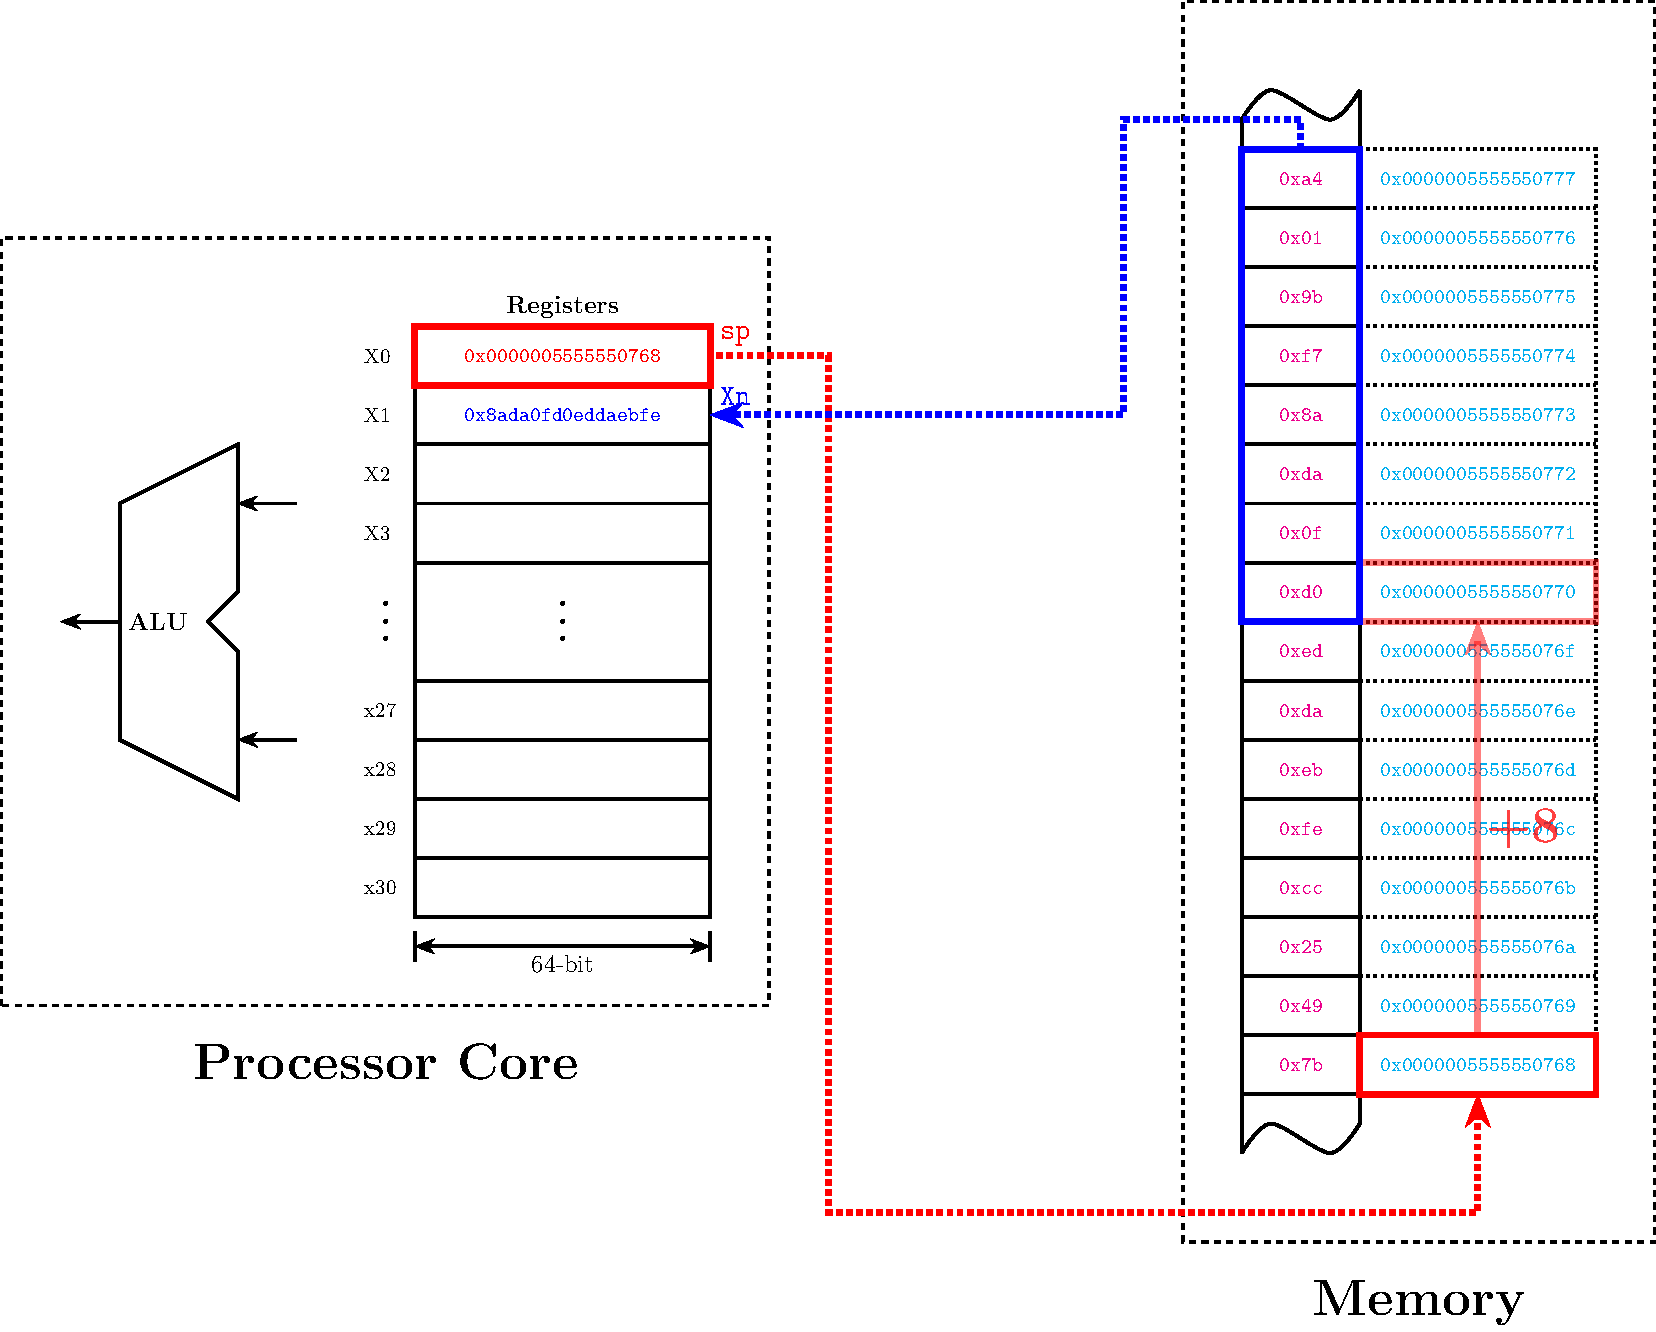
\includegraphics[width=\textwidth]{architectures/immediate-offset.pdf}
	\caption{Signed Immediate Offset.}
\end{figure}

\begin{table}[h!]\setstretch{1.25}\centering
\caption{Pre-index, Post-index and Pre-index with Update}
\resizebox*{1\textwidth}{!}{\begin{tabular}{l|l}
	\toprule[1.2pt]
	\multirow{3}{*}{\textbf{Pre-index}} & \texttt{ldr\hspace{1cm} X1,\ [X0, \#0x08]} \\ \cline{2-2}
	& \texttt{X1 $\gets$ memory.word[X0 + 0x08]} \\
	& \texttt{X0} remains unchanged \\ \hline
	\multirow{3}{*}{\textbf{Post-index}} & \texttt{ldr\hspace{1cm} X1,\ [X0],\ \#0x08} \\ \cline{2-2}
	& \texttt{X1 $\gets$ memory.word[X0]} \\
	& \texttt{X0 $\gets$ X0 + 0x08} \\ \hline
	\multirow{3}{*}{\textbf{Pre-index with Update}} & \texttt{ldr\hspace{1cm} X1,\ [X0, \#0x08]!} \\ \cline{2-2}
	& \texttt{X1 $\gets$ memory.word[X0 + 0x08]} \\
	& \texttt{X0$\gets$ X0 + 0x08}\\
	\bottomrule[1.2pt]
\end{tabular}}
\end{table}

\newpage
\subsection{Load and Store Instructions}
The load and store instructions allow the programmer to move data from memory to registers
or from registers to memory. The load/store instructions can be grouped into the following
types:
\begin{itemize}
	\item single register,
	\item register pair,
	\item atomic.
\end{itemize}

\subsubsection{Load/store single register}
These instructions transfer a double-word(64-bit), single word(32-bit), half-word(16-bit), or byte(8-bit) from a register to memory or from memory to a register:

\begin{table}[h!]
\begin{tabular}{ll}
	\texttt{\bf ldr} & Load Register \\
	\texttt{\bf str} & Store Register
\end{tabular}
\end{table}

\begin{figure}[h!]\centering
	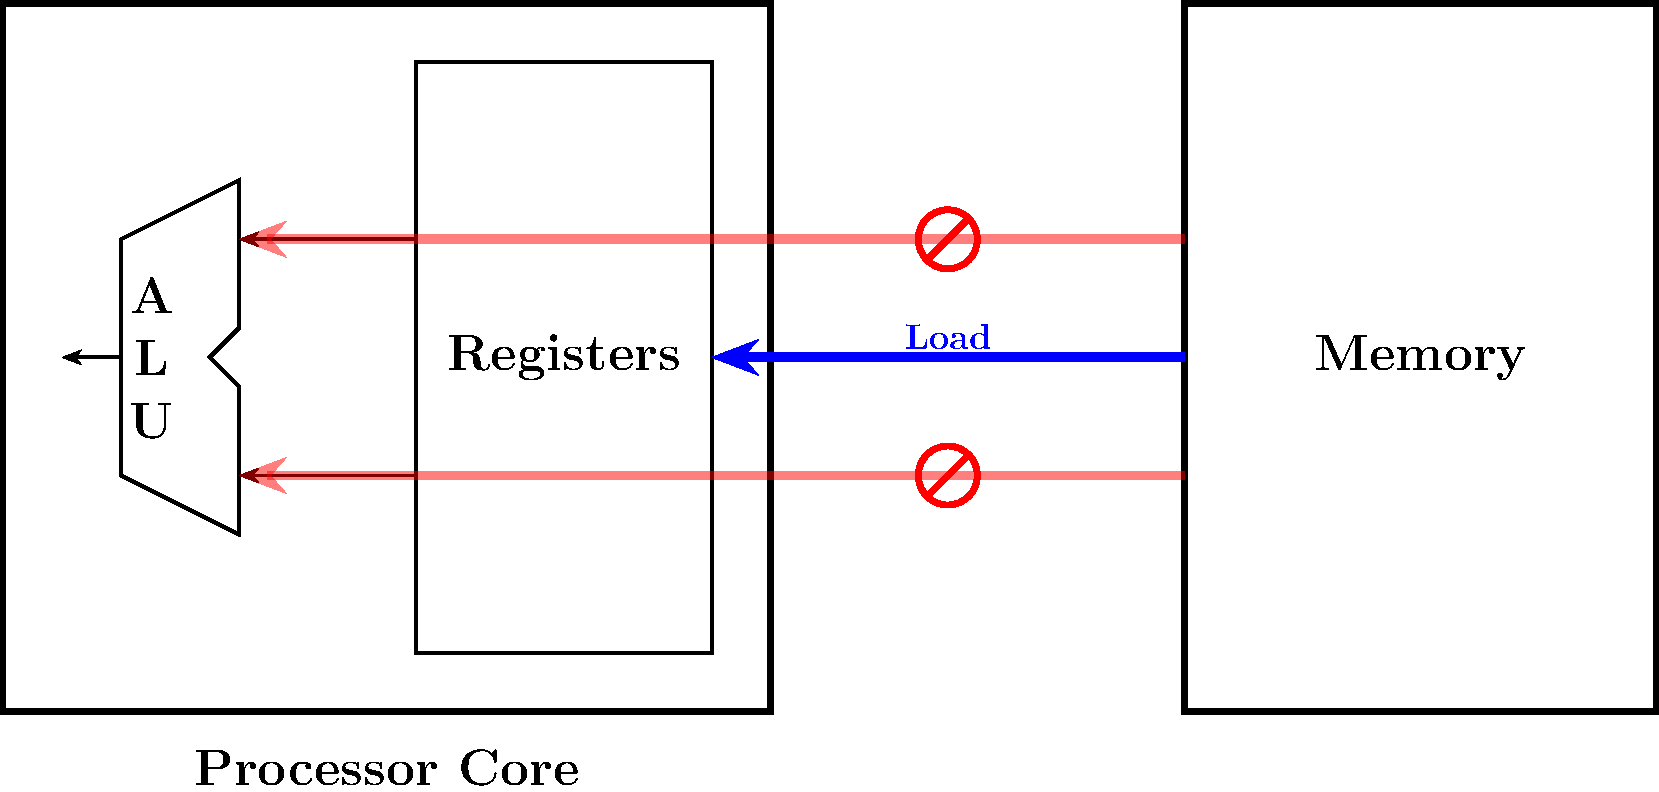
\includegraphics[width=.975\textwidth]{architectures/load.pdf}
	\caption{Loading Data from Memory}
\end{figure}

\begin{figure}[h!]\centering
	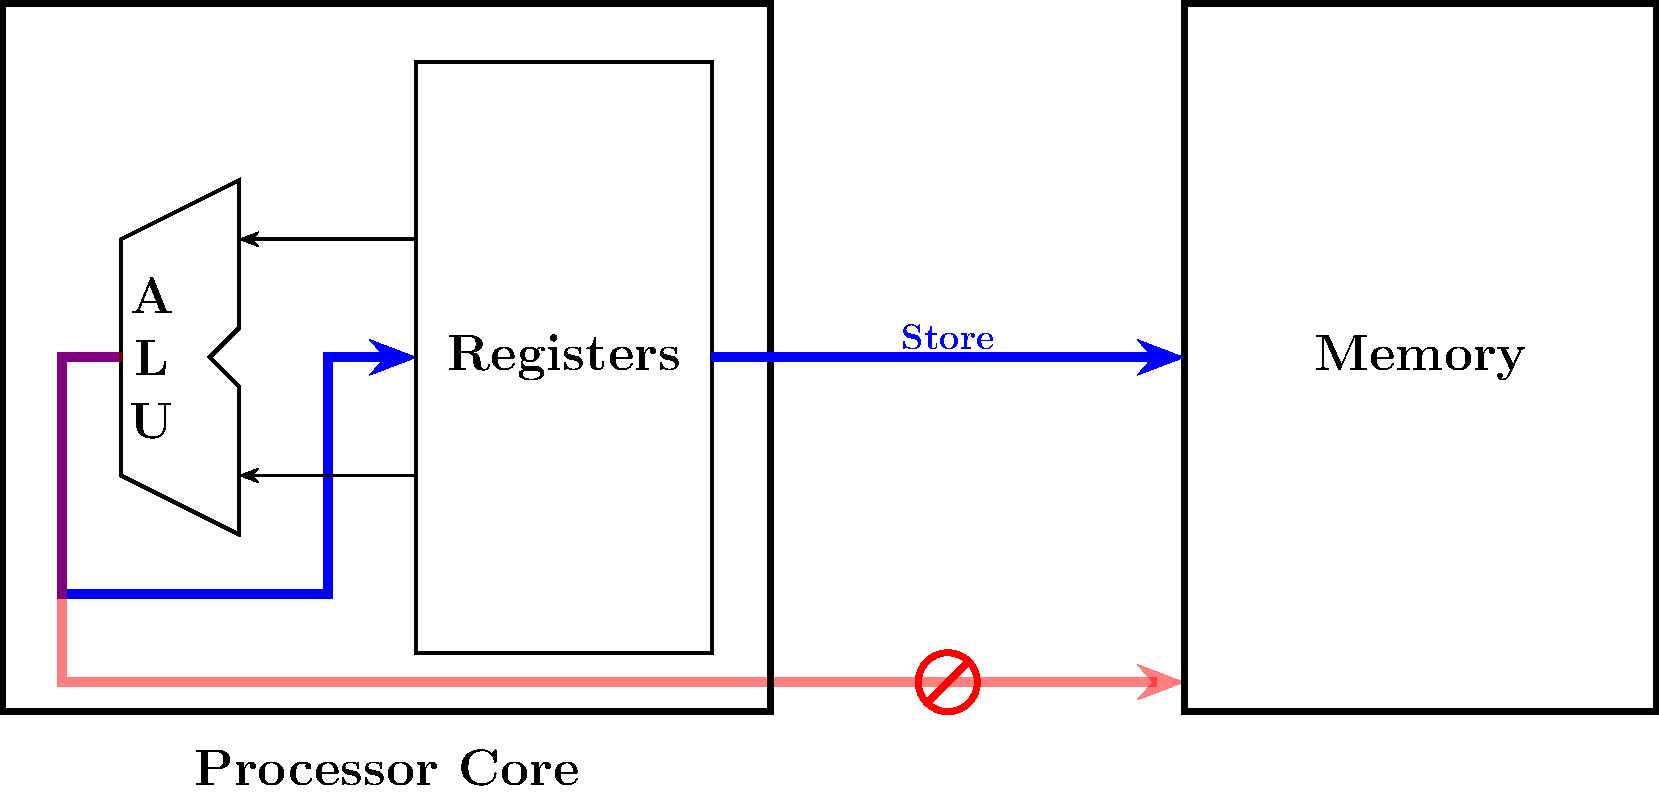
\includegraphics[width=.975\textwidth]{architectures/store.pdf}
	\caption{Storing Data to Memory}
\end{figure}

\newpage
\begin{description}
	\item[Syntax] \boxed{\texttt{<op>\{<size>\}\hspace{.5cm} Rd, <addr>}}
	\nonumsidenote{\begin{itemize}[leftmargin=*]
			\item \texttt{<op>} is either \texttt{ldr} or \texttt{str}.
			\item The optional \texttt{<size>} is one of: \begin{center}
			\ttfamily b,\quad h,\quad sb,\quad sh,\quad sw
			\end{center}
			\item[] \texttt{b}: unsigned byte
			\item[] \texttt{h}: unsigned half-word
			\item[] \texttt{sb}: signed byte
			\item[] \texttt{sh}: signed half-word
			\item[] \texttt{sw}: signed word
			\item \texttt{str} cannot use a singed \texttt{<size>}. It also cannot use the literal addressing mode.
	\end{itemize}}
	\item[Operation] \ \begin{table}[h!]
		\begin{tabular}{lll}
			\textbf{Name} & \textbf{Effect} & \textbf{Description} \\ \hline
			\texttt{ldr} & \texttt{Rd $\gets$ Mem[addr]} & Load register from memory at \texttt{addr} \\ \hline
			\texttt{str} & \texttt{Mem[addr] $\gets$ Rd} & Store register in memory at \texttt{addr}
		\end{tabular}
	\end{table}
\end{description}

\begin{example*} \ \\ 
\begin{lstlisting}
	// Load the word (4 byte) value
	// from Mem[x4] into w8,
	// and set the upper four bytes of x8to zero.
	ldr		w8, [x4]
\end{lstlisting}
\begin{figure}[h!]\centering
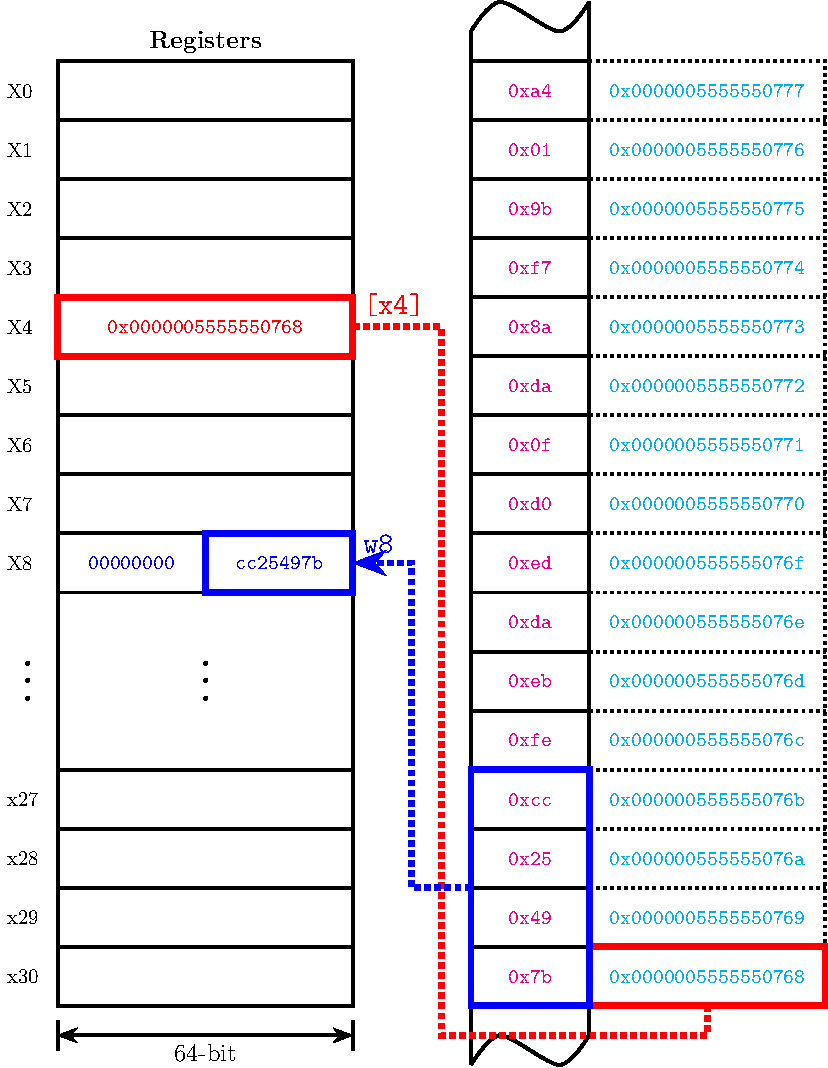
\includegraphics[width=.9\textwidth]{architectures/load-store-example1.pdf}
\caption{Load the word (4 byte) value from \texttt{Mem[x4]} into \texttt{w8}, and set the upper four bytes of \texttt{x8} to zero.}	
\end{figure}
\newpage
\begin{lstlisting}
	// Store the least-significant byte
	// from register x12 into Mem[x2].
	strb		x12, [x2]
\end{lstlisting}
\begin{lstlisting}
	// Load the double-word (8 byte) value
	// from Mem[x3 + 7] into x5. Then set x3 = x3 + 7:
	ldr		x5, [x3, #7]!
\end{lstlisting}
\begin{lstlisting}
	// Store the half-word (2 byte) value
	// in w9 to Mem[x6]. Then set x6 = x6 + 7:
	strh		w9, [x6], #7
\end{lstlisting}
\begin{lstlisting}
	// Load the half-word value
	// from Mem[x0 + 8] into x5 and sign extend it:
	ldrsh		x5, [x0, 8]
\end{lstlisting}
\begin{lstlisting}
	// Store the least significant byte
	// in w1 at Mem[x9]:
	strb		w1, [x9]
\end{lstlisting}
\end{example*}

\subsubsection{Load/store single register (unscaled)}
These instructions are the same as Load/Store Single Register, except that they only use an
unscaled, signed addressing mode with an offset range of $\intcc{-256,256}$. \nonumsidenote{Programmers rarely need to write \texttt{ldur} or \texttt{stur} explicitly. The programmer can just use \texttt{ldr} or \texttt{str}, and the assembler will almost always automatically convert them to \texttt{ldur} or \texttt{stur} when appropriate.}
\begin{table}[h!]
	\begin{tabular}{ll}
		\texttt{\bf ldur} & Load Register (Unscaled) \\
		\texttt{\bf stur} & Store Register (Unscaled)
	\end{tabular}
\end{table}
\begin{description}
\item[Syntax] \boxed{\texttt{<op>\{<size>\}\hspace{.5cm} Rd, [Xn, \#imm9]}}
\item[Operation] \ \begin{table}[h!]
	\begin{tabular}{lll}
		\textbf{Name} & \textbf{Effect} & \textbf{Description} \\ \hline
		\texttt{ldur} & \texttt{Rd $\gets$ Mem[addr]} & Load register from memory at \texttt{addr} \\ \hline
		\texttt{stur} & \texttt{Mem[addr] $\gets$ Rd} & Store register in memory at \texttt{addr}
	\end{tabular}
\end{table}
\end{description}
\begin{example*}
\ \begin{lstlisting}
	// Load the byte value from Mem[x5 + 255]. 
	// Sign extend it and store the value in x4:
	ldursb		x4, [x5, #255]
\end{lstlisting}
\begin{lstlisting}
	// Store the double-word value in x1 to Mem[x2 - 256]:
	stur		x1, [x2, #-256]
\end{lstlisting}
\end{example*}

\subsubsection{Load/store pair}
These instructions are used to store or load two registers at a time. This can be useful for moving registers onto the stack or for copying data. These two instructions are particularly useful for transferring data in a load-store architecture because each instruction can move twice as much information as the \texttt{ldr} and \texttt{str} instructions.

\begin{table}[h!]
	\begin{tabular}{ll}
		\texttt{\bf ldp} & Load Pair \\
		\texttt{\bf stp} & Store Pair
	\end{tabular}
\end{table}
\begin{description}
	\item[Syntax] \boxed{\texttt{<op>\{<size>\}\hspace{.5cm} Rt, Rt2, <addr>}}
	\nonumsidenote{\begin{itemize}[leftmargin=*]
			\item \texttt{<op>} is either \texttt{ldp} or \texttt{stp}.
			\item The optional \texttt{<size>} is optionally \texttt{sw} for signed words.
			\item \texttt{<addr>} is 7 bits Pre-indexed, Post-indexed, or Signed immediate.
			\item Signed immediate
			\item[] \texttt{Xt} range: $[\texttt{-0x200, 0x1f8}]$.
			\item[] \texttt{Wt} range: $[\texttt{-0x100, 0xfc}]$.
	\end{itemize}}
	\item[Operation] \ \begin{table}[h!]
		\begin{tabular}{lll}
			\textbf{Name} & \textbf{Effect} & \textbf{Description} \\ \hline
			\multirow{5}{*}{\texttt{ldp}} & & Load register pair\\
			& \texttt{Rt $\gets$ Mem[addr]}&  from memory at \texttt{addr}\\
			& \texttt{Rt2 $\gets$ Mem[addr + size(Rt)]} & where \texttt{sizeof(Rt)} is \\
			& & 4 for \texttt{Wt} registers \\
			& & and 8 for \texttt{Xt} registers \\ \hline
			\multirow{2}{*}{\texttt{stur}} & \texttt{Mem[addr] $\gets$ Rd} & Store register pair \\
			& \texttt{Mem[addr + size(Rt)] $\gets$ Rt2} & in memory at \texttt{addr}
		\end{tabular}
	\end{table}
\end{description}
\begin{example*}
	\ \begin{lstlisting}
		// Load the byte value from Mem[x5 + 255]. 
		// Sign extend it and store the value in x4:
		ldursb		x4, [x5, #255]
	\end{lstlisting}
	\begin{lstlisting}
		// Store the double-word value in x1 to Mem[x2 - 256]:
		stur		x1, [x2, #-256]
	\end{lstlisting}
\end{example*}

\subsubsection{Summary}

\newpage
\subsection{Branch instructions}
Branch instructions allow the programmer to change the address of the next instruction to be
executed. They are used to implement loops, if-then structures, subroutines, and other flow
control structures. There are five instructions related to branching:
\begin{itemize}
	\item Branch,
	\item Branch to Register,
	\item Branch and Link (subroutine call),
	\item Compare and Branch, and
	\item Form program-counter-relative Address.
\end{itemize}

\subsubsection{Branch}